% Created by tikzDevice version 0.10.1 on 2017-03-27 16:29:12
% !TEX encoding = UTF-8 Unicode
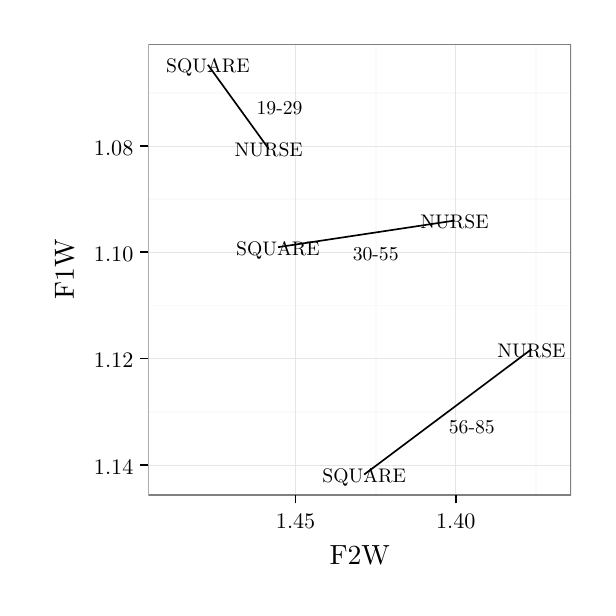
\begin{tikzpicture}[x=1pt,y=1pt]
\definecolor{fillColor}{RGB}{255,255,255}
\path[use as bounding box,fill=fillColor,fill opacity=0.00] (0,0) rectangle (202.36,202.36);
\begin{scope}
\path[clip] (  0.00,  0.00) rectangle (202.36,202.36);
\definecolor{drawColor}{RGB}{255,255,255}
\definecolor{fillColor}{RGB}{255,255,255}

\path[draw=drawColor,line width= 0.6pt,line join=round,line cap=round,fill=fillColor] (  0.00,  0.00) rectangle (202.36,202.36);
\end{scope}
\begin{scope}
\path[clip] ( 43.58, 33.48) rectangle (196.36,196.36);
\definecolor{fillColor}{RGB}{255,255,255}

\path[fill=fillColor] ( 43.58, 33.48) rectangle (196.36,196.36);
\definecolor{drawColor}{gray}{0.98}

\path[draw=drawColor,line width= 0.6pt,line join=round] ( 43.58,178.81) --
	(196.36,178.81);

\path[draw=drawColor,line width= 0.6pt,line join=round] ( 43.58,140.40) --
	(196.36,140.40);

\path[draw=drawColor,line width= 0.6pt,line join=round] ( 43.58,101.99) --
	(196.36,101.99);

\path[draw=drawColor,line width= 0.6pt,line join=round] ( 43.58, 63.58) --
	(196.36, 63.58);

\path[draw=drawColor,line width= 0.6pt,line join=round] (183.62, 33.48) --
	(183.62,196.36);

\path[draw=drawColor,line width= 0.6pt,line join=round] (125.75, 33.48) --
	(125.75,196.36);
\definecolor{drawColor}{gray}{0.90}

\path[draw=drawColor,line width= 0.2pt,line join=round] ( 43.58,159.61) --
	(196.36,159.61);

\path[draw=drawColor,line width= 0.2pt,line join=round] ( 43.58,121.19) --
	(196.36,121.19);

\path[draw=drawColor,line width= 0.2pt,line join=round] ( 43.58, 82.78) --
	(196.36, 82.78);

\path[draw=drawColor,line width= 0.2pt,line join=round] ( 43.58, 44.37) --
	(196.36, 44.37);

\path[draw=drawColor,line width= 0.2pt,line join=round] (154.69, 33.48) --
	(154.69,196.36);

\path[draw=drawColor,line width= 0.2pt,line join=round] ( 96.82, 33.48) --
	( 96.82,196.36);
\definecolor{drawColor}{RGB}{0,0,0}

\node[text=drawColor,anchor=base,inner sep=0pt, outer sep=0pt, scale=  0.71] at (182.06, 83.25) {NURSE};

\node[text=drawColor,anchor=base,inner sep=0pt, outer sep=0pt, scale=  0.71] at (121.58, 37.94) {SQUARE};

\node[text=drawColor,anchor=base,inner sep=0pt, outer sep=0pt, scale=  0.71] at (154.27,129.72) {NURSE};

\node[text=drawColor,anchor=base,inner sep=0pt, outer sep=0pt, scale=  0.71] at ( 90.45,120.10) {SQUARE};

\node[text=drawColor,anchor=base,inner sep=0pt, outer sep=0pt, scale=  0.71] at ( 87.10,155.63) {NURSE};

\node[text=drawColor,anchor=base,inner sep=0pt, outer sep=0pt, scale=  0.71] at ( 65.12,186.01) {SQUARE};

\path[draw=drawColor,line width= 0.6pt,line join=round] (182.06, 86.19) --
	(121.58, 40.88);

\path[draw=drawColor,line width= 0.6pt,line join=round] (154.27,132.66) --
	( 90.45,123.04);

\path[draw=drawColor,line width= 0.6pt,line join=round] ( 87.10,158.57) --
	( 65.12,188.95);

\node[text=drawColor,anchor=base,inner sep=0pt, outer sep=0pt, scale=  0.71] at (160.48, 55.83) {56-85};

\node[text=drawColor,anchor=base,inner sep=0pt, outer sep=0pt, scale=  0.71] at (125.75,118.25) {30-55};

\node[text=drawColor,anchor=base,inner sep=0pt, outer sep=0pt, scale=  0.71] at ( 91.03,171.07) {19-29};
\definecolor{drawColor}{gray}{0.50}

\path[draw=drawColor,line width= 0.6pt,line join=round,line cap=round] ( 43.58, 33.48) rectangle (196.36,196.36);
\end{scope}
\begin{scope}
\path[clip] (  0.00,  0.00) rectangle (202.36,202.36);
\definecolor{drawColor}{RGB}{0,0,0}

\node[text=drawColor,anchor=base east,inner sep=0pt, outer sep=0pt, scale=  0.80] at ( 38.18,156.30) {1.08};

\node[text=drawColor,anchor=base east,inner sep=0pt, outer sep=0pt, scale=  0.80] at ( 38.18,117.89) {1.10};

\node[text=drawColor,anchor=base east,inner sep=0pt, outer sep=0pt, scale=  0.80] at ( 38.18, 79.48) {1.12};

\node[text=drawColor,anchor=base east,inner sep=0pt, outer sep=0pt, scale=  0.80] at ( 38.18, 41.06) {1.14};
\end{scope}
\begin{scope}
\path[clip] (  0.00,  0.00) rectangle (202.36,202.36);
\definecolor{drawColor}{RGB}{0,0,0}

\path[draw=drawColor,line width= 0.6pt,line join=round] ( 40.58,159.61) --
	( 43.58,159.61);

\path[draw=drawColor,line width= 0.6pt,line join=round] ( 40.58,121.19) --
	( 43.58,121.19);

\path[draw=drawColor,line width= 0.6pt,line join=round] ( 40.58, 82.78) --
	( 43.58, 82.78);

\path[draw=drawColor,line width= 0.6pt,line join=round] ( 40.58, 44.37) --
	( 43.58, 44.37);
\end{scope}
\begin{scope}
\path[clip] (  0.00,  0.00) rectangle (202.36,202.36);
\definecolor{drawColor}{RGB}{0,0,0}

\path[draw=drawColor,line width= 0.6pt,line join=round] (154.69, 30.48) --
	(154.69, 33.48);

\path[draw=drawColor,line width= 0.6pt,line join=round] ( 96.82, 30.48) --
	( 96.82, 33.48);
\end{scope}
\begin{scope}
\path[clip] (  0.00,  0.00) rectangle (202.36,202.36);
\definecolor{drawColor}{RGB}{0,0,0}

\node[text=drawColor,anchor=base,inner sep=0pt, outer sep=0pt, scale=  0.80] at (154.69, 21.47) {1.40};

\node[text=drawColor,anchor=base,inner sep=0pt, outer sep=0pt, scale=  0.80] at ( 96.82, 21.47) {1.45};
\end{scope}
\begin{scope}
\path[clip] (  0.00,  0.00) rectangle (202.36,202.36);
\definecolor{drawColor}{RGB}{0,0,0}

\node[text=drawColor,anchor=base,inner sep=0pt, outer sep=0pt, scale=  1.00] at (119.97,  8.40) {F2W};
\end{scope}
\begin{scope}
\path[clip] (  0.00,  0.00) rectangle (202.36,202.36);
\definecolor{drawColor}{RGB}{0,0,0}

\node[text=drawColor,rotate= 90.00,anchor=base,inner sep=0pt, outer sep=0pt, scale=  1.00] at ( 16.67,114.92) {F1W};
\end{scope}
\end{tikzpicture}
